%%%%%%%%%%%%%%%%%%%%%%%%%%%%%%%%%%%%%%%%%
% Short Three-Column Newsletter
% LaTeX Template
% Version 1.0 (11/9/13)
%
% Original author:
% Frits Wenneker (http://www.howtotex.com) 
% With extensive modifications by:
% Vel (vel@latextemplates.com)
% 
% This template has been downloaded from:
% http://www.LaTeXTemplates.com
%
% License:
% CC BY-NC-SA 3.0 (http://creativecommons.org/licenses/by-nc-sa/3.0/)
%
%%%%%%%%%%%%%%%%%%%%%%%%%%%%%%%%%%%%%%%%%

%----------------------------------------------------------------------------------------
%	PACKAGES AND DOCUMENT CONFIGURATIONS
%----------------------------------------------------------------------------------------

\documentclass[10pt,a4paper]{article} % Paper type (a4paper, usletter or legal) and font size (10, 11 or 12)

\setlength\topmargin{-48pt} % Top margin
\setlength\headheight{0pt} % Header height
\setlength\textwidth{7.0in} % Text width
\setlength\textheight{9.5in} % Text height
\setlength\oddsidemargin{-30pt} % Left margin
\setlength\evensidemargin{-30pt} % Left margin (even pages) - only relevant with 'twoside' article option

\usepackage{charter} % Charter font for main content

\frenchspacing % Reduces space after periods to make text more compact for a three-column layout

\usepackage{graphicx} % Required for including images
\usepackage{amssymb,amsmath} % Math packages
\usepackage{multicol} % Required for the three-column layout of the document
\usepackage{url} % Clickable links
\usepackage{enumitem} % Reduces the amount of space within and between lists with [noitemsep,nolistsep]
\usepackage{marvosym} % Required for the use of symbols
\usepackage{wrapfig} % Allows wrapping text around figures
\usepackage[T1]{fontenc} % Use 8-bit encoding that has 256 glyphs
\usepackage{datetime} % Required for defining a custom date style
\newdateformat{mydate}{\monthname[\THEMONTH] \THEYEAR} % Set a custom date format
\usepackage[pdfpagemode=FullScreen, colorlinks=false]{hyperref} % Link colors and PDF behavior in Acrobat
\usepackage{fancyhdr} % Required to define custom headers/footers
\pagestyle{fancy} % Enables the custom headers/footers for all pages following this

% ----- Added Sam - BEGIN
\usepackage[utf8]{inputenc} %Support for ie. Umlauts
\usepackage[english,ngerman]{babel} %Füre deutsch Dokument, Datumformat
\usepackage{verbatim} %Allows the use of comments
\usepackage{color}
% ----- Added Sam - END

\usepackage{tcolorbox} % See: http://get-software.net/macros/latex/contrib/tcolorbox/tcolorbox.pdf

\newtcolorbox{shortExplainedBox}[1]{colback=blue!10!white,colframe=blue!55!black,fonttitle=\bfseries,title=#1}

\newtcolorbox{invitationBox}[1]{colback=red!10!white,colframe=red!55!black,fonttitle=\bfseries,title=#1}

%-----------------------------------------------------------
% Header and footer
\lfoot{\footnotesize % Left footer containing newsletter contact information
ZHAW - Angewandte Kryptografie - Fallstudie - E-Voting: Ja oder Nein? \\
Gruppe Diffie: Daniel Brun, Samuel Baumgartner, Michael Hadorn, Simon Lang
%\Mundus\ \href{http://www.LaTeXTemplates.com}{LaTeXTemplates.com} \quad
%\Telefon\ (000) 111-1111 \quad
%\Letter\ \href{mailto:email@email.com}{email@email.com}
}

\cfoot{} % Empty center footer

\rfoot{\footnotesize ~\\ Seite \thepage} % Right footer - page counter

\renewcommand{\headrulewidth}{0.0pt} % No horizontal rule for the header
\renewcommand{\footrulewidth}{0.4pt} % Horizontal rule separating the footer from the document
%-----------------------------------------------------------

%-----------------------------------------------------------
% Define separators
\newcommand{\HorRule}[1]{\noindent\rule{\linewidth}{#1}} % Creates a horizontal rule
\newcommand{\SepRule}{\noindent	% Creates a shorter separator rule
\begin{center}
\rule{250pt}{1pt} % Page width and rule width
\end{center}
}
%-----------------------------------------------------------

%-----------------------------------------------------------
% Define title and article styles
\newcommand{\NewsletterName}[1]{ % Newsletter title
\begin{center}
\Huge \usefont{T1}{fvs}{b}{n} % Use the Bera Sans Bold font
#1
\end{center}	
\par \normalsize \normalfont}

\newcommand{\JournalIssue}[1]{ % Date and issue number at the top of the newsletter
\hfill \textsc{\mydate \today} % Right-aligned date and issue number
\par \normalsize \normalfont}

\newcommand{\NewsItem}[1]{ % News item title
\usefont{T1}{fvs}{n}{n} % Use the Bera Sans Normal font
\vspace{24pt}\large #1\vspace{3pt} % Print the title with space around it in a larger font size
\par \normalsize \normalfont}

\newcommand{\NewsAuthor}[1]{ % Author name under the item title
\hfill by \textsc{#1} \vspace{20pt} % Right-aligned author name in small caps with space after it
\par \normalfont}		

%----------------------------------------------------------------------------------------
%	TITLE
%----------------------------------------------------------------------------------------

\begin{document}

\JournalIssue{4} % Issue number

\NewsletterName{E-Voting: Ja oder Nein?} % Newsletter title

\noindent\HorRule{3pt} \\[-0.75\baselineskip] % Thick horizontal rule
\HorRule{1pt} % Thin horizontal rule

%----------------------------------------------------------------------------------------
%	MAIN NEWS ITEM
%----------------------------------------------------------------------------------------

\vspace{0.5cm}
\SepRule
\vspace{-0.5cm}

%todo: bildquelle?!
\begin{center}
\begin{minipage}[h]{0.75\linewidth}
\begin{wrapfigure}{l}{0.4\textwidth}

\includegraphics[width=0.4\textwidth]{images/e-vote-1_cut.jpg}
\\
\end{wrapfigure}

\NewsItem{Abstimmungswochenende, 1995} % Main next item title
\vspace{3pt} % Some extra whitespace since there is no author as for the news in the body of the newsletter
\begin{quotation} % Example of a quotation
\noindent{\Huge``}

\noindent\normalsize\textit{Huch ja, abstimmen - muss ich auch noch. Wird aber ganz schön knapp, wenn ich bis Sonntagmittag zur Gemeinde muss. Wann hat die überhaupt geöffnet?\\
Ach wie schön es doch wäre, wenn mir der Weg zur Gemeinde gespart bleiben würde.
Ich stelle mir eine Welt vor, in der man ohne Aufwand von überall her, unabhängig von Öffnungszeiten, sein Wahl abgeben könnte.}

\hfill{\Huge''}

\hfill-- fiktive Person, im Jahr 1995
\end{quotation}

%\par\hfill --- Michael Hadorn
\end{minipage}
\end{center}

\vspace{0.5cm}
\SepRule % Small horizontal rule after the main news item
\vspace{0.5cm}

%\setlength{\columnsep}{16pt} % Uncomment to manually change the white space between columns
\begin{multicols}{3} % Begin the three-column layout

%----------------------------------------------------------------------------------------
%	OTHER NEWS
%----------------------------------------------------------------------------------------

\begin{flushleft}
\NewsItem{Auswirkungen und Nebenwirkungen}
\end{flushleft}
%\NewsAuthor{Samuel Baumgartner}

Wird die Art wie man abstimmt massgebend geändert, stellt sich die Frage ob das Verhalten der Wähler dadurch beeinflusst wird, gewollt oder ungewollt. So hat sich z.B. gezeigt, dass das Ändern der Abstimmungstechnologie zu einer Verminderung der ungültigen Stimmen führt. Auch kann sich das Vertrauen in die Abstimmungstechnologie bei einer massgebenden Umstellung ändern und sich sogar auf das Abstimmungsergebnis auswirken.
Es ist wichtig die Effekte und vor allem auch die Nebeneffekte, welches ein Einführen einer neuen Abstimmungstechnologie mit sich bringt, zu analysieren.

Haben Sie sich schon mal gefragt warum der wichtigste Kandidat einer Partei immer ganz oben auf der Liste steht? Hat dies einen Einfluss? Es gibt Methoden wie die Robson Rotation, welche sicherstellt, dass keine Kandidaten bevorzugt werden.
Interessiert Sie was passieren würde, wenn es keine Listen bei der Wahl des Regierungsrates mehr gäbe und jeder gezwungen wäre seine eigene Liste zu erstellen. (95\% der Wähler stimmen anhand der vorgegeben Listen)

Die interessanteste Frage ist jedoch, ob ein Wähler der elektronisch stimmt, anders wählt als eine Person die auf Papier stimmt. Was wir Ihnen bereits jetzt verraten können: Es gibt einen Unterschied! Wo dieser Unterscheid liegt, ob er sich auf das Abstimmungsergebnis auswirkt und ob sich diese Frage überhaupt abschliessend beantworten lässt, erfahren sie an unserem Anlass.

Eine besonders interessante und auch positive Auswirkung von E-Votings ist ein Anstieg der Expressivität. Man erkannte, dass bei einer elektronischen Abstimmung mehr Präferenzen angegeben wurden als bei einer Papier-Wahl. So ist die Wahrscheinlichkeit höher, dass ein Wähler seine Präferenz für alle Kandidaten abgibt als nur für seine präferierte Partei.


%----------------------------------------------------------------------------------------
%	Invitation box
%----------------------------------------------------------------------------------------

\begin{invitationBox}{Symposium \\E-Voting: Ja oder Nein?}
\begin{tabular}{r p{4cm}}
Wann: & 10. Dezember 2014,\newline ab 19:00 Uhr \\
Wo: &  
\end{tabular}
\end{invitationBox}

%-----------------------------------------------------------

\begin{flushleft}
\NewsItem{Voraussetzungen und Entwicklung}
\end{flushleft}
% https://docs.google.com/document/d/112u5nT_h6aL9lLoVC8Snh4IpzxSJY7eKY2roOVor_lE/edit
%---Dummy-Text
Lorem ipsum dolor sit amet, consetetur sadipscing elitr, sed diam nonumy eirmod tempor invidunt ut labore et dolore magna aliquyam erat, sed diam voluptua. At vero eos et accusam et justo duo dolores et ea rebum. Stet clita kasd gubergren, no sea takimata sanctus est Lorem ipsum dolor sit amet. Lorem ipsum dolor sit amet, consetetur sadipscing elitr, sed diam nonumy eirmod tempor invidunt ut labore et dolore magna aliquyam erat, sed diam voluptua. At vero eos et accusam et justo duo dolores et ea rebum. Stet clita kasd gubergren, no sea takimata sanctus est Lorem ipsum dolor sit amet. Lorem ipsum dolor sit amet, consetetur sadipscing elitr, sed diam nonumy eirmod tempor invidunt ut labore et dolore magna aliquyam erat, sed diam voluptua. At vero eos et accusam et justo duo dolores et ea rebum. Stet clita kasd gubergren, no sea takimata sanctus est Lorem ipsum dolor sit amet.   

Duis autem vel eum iriure dolor in hendrerit in vulputate velit esse molestie consequat, vel illum dolore eu feugiat nulla facilisis at vero eros et accumsan et iusto odio dignissim qui blandit praesent luptatum zzril delenit augue duis dolore te feugait nulla facilisi. Lorem ipsum dolor sit amet, consectetuer adipiscing elit, sed diam nonummy nibh euismod tincidunt ut laoreet dolore magna aliquam erat volutpat.   

Ut wisi enim ad minim veniam, quis nostrud exerci tation ullamcorper suscipit lobortis nisl ut aliquip ex ea commodo consequat. Duis autem vel eum iriure dolor in hendrerit in vulputate velit esse molestie consequat, vel illum dolore eu feugiat nulla facilisis at vero eros et accumsan et iusto odio dignissim qui blandit praesent luptatum zzril delenit augue duis dolore te feugait nulla facilisi.   

Nam liber tempor cum soluta nobis eleifend option congue nihil imperdiet doming id quod mazim placerat facer



\end{multicols} % End the three-column layout for a large picture

% TODO: Dani: Definition e- / i-Voting
\begin{center}
\vspace{10pt}
\begin{shortExplainedBox}{Kurz erklärt: E-Voting und i-Voting}
Beim klassischen Wahlsystem gibt jeder Wähler seine Stimme entweder via Brief-Post oder direkt in einem Wahllokal ab. E-Voting (electronic-Voting) bezeichnet ein Wahlsystem, bei dem zur Erfassung, Speicherung, Verarbeitung, Auswertung oder Weiterleitung in irgendeiner Weise Informationstechnologien zum Einsatz kommen. Dazu zählen unter anderem Web Polls, Elektronische Wahlgeräte, Wahl mittels Wahlkiosken, E-Counting und i-Voting.
\newline\newline
\textbf{Web-Polls}\\
Abstimmungen auf Web-Seiten. Diese garantieren jedoch die Korrektheit des Wahlergebnisses und die Einhaltung der Anonymität nicht. Für ernsthafte Wahlen können diese nicht in Betracht gezogen werden.\\

\textbf{Elektronische Wahlgeräte}\\
Die Wahl erfolgt auf einem elektronischen Gerät in einem Wahllokal. Da die Geräte untereinander nicht vernetzt sind, müssen die Ergebnisse manuell addiert werden.\\

\textbf{Elektronische Wahl mit Wahlkiosken}\\
An Wahlkiosken können die Stimmberechtigten analog den elektronischen Wahlgeräten Ihre Stimme abgeben. Die Wahlkioske sind untereinander vernetzt. Durch die Vernetzung müssen die einzelnen Ergebnisse nicht manuell addiert werden.\\

\textbf{E-Counting}\\
Die Wahl erfolgt auf speziellen Wahlzetteln, welche anschliessend von eingescannt und mit Hilfe einer Texterkennungssoftware erfasst.\\

\textbf{i-Voting}\\
Beim i-Voting (internet-Voting) erfolgt die Stimmabgabe von einem beliebigen Computer mit Internetverbindung. Dabei kommen entweder Online-Portale, E-Mail-Clients oder spezielle Voting-Software zum Einsatz.\\
\end{shortExplainedBox}
\vspace{10pt}
\end{center}

\begin{multicols}{3} % Continue the three-column layout



%-----------------------------------------------------------
\begin{flushleft}
\NewsItem{Sicherheitsprobleme}
\end{flushleft}

\textbf{Italian Attack}

Bei elektronischen Abstimmungen müssen die gesamten Abstimmungsdaten bzw. Wahlzettel offen gelegt werden um auditiert werden zu können. Zwar sind diese Daten anonymisiert, lassen aber immer noch den sogenannten 'Italian Attack' zu. Hierbei kann eine Person, welche sich Stimmen gekauft hatte oder Wähler zu einer gewissen Wahl gezwungen hatte, kontrollieren ob diese Aktion erfolgreich war.

\textbf{Kompromittierte Clients}

\textcolor{red}{TODO: Inhalt (Wer macht das?)}

%-----------------------------------------------------------

% glossary: Keys (private, public), unique votingcard number (UVN)
\begin{flushleft}
\NewsItem{Genf}
\end{flushleft}

%\NewsAuthor{Michael Hadorn}
Seit 2003 wird in Genf eine E-Voting Lösung angeboten. Es handelt sich um eine Eigenentwicklung, die extra für Genf entwickelt wurde.
Folgend wird auf die einzelnen Schritte des Abstimmungsprozesses, konkret bei diesem System in Genf, eingegangen.
\\\\
\textbf{Die Initialisierung}
\\
Initial muss die elektronische Stimmbox erstellt werden.
Um die Daten zu verschlüsseln und später wieder zu entschlüsseln, müssen verschiedene Passwörter und Keys definiert werden.

Dazu wird das bewährte ``Public - private Key'' Prinzip verwendet.
Es werden zwei verschiedene Schlüssel erstellt.
Die Daten werden mit dem public Key verschlüsselt, und sind nur mit dem private Key wieder entschlüsselbar.
Der private Key wird mit zwei Passwörter (aus zwei verschiedenen Gruppen) verschlüsselt.
Daraus folgt, dass man die effektiven Wahlergebnisse nur mit dem Einverständnis beider Passwortbesitzer-Gruppen einsehen kann.
Das Wissen von nur einem Passwort ist somit wertlos.

Da ohne private Key keinen Zugriff auf die Daten möglich ist, werden alle Daten mindenstens auf zwei verschiedenen Medien gesichert. Auch die Passwörter werden in einem Umschlag auf dem Notaramt hinterlegt.
Der Computer der für die Generierung der Passwörter verwendet wird und auf dem der ganze Prozess eingeleitet wird, wird verschlossen und versiegelt aufbewahrt.
\\\\
\textbf{Der Wahlvorgang}
\\
Der konkrete Wahlvorgang läuft nun wie folgt ab:\\
Jeder Stimmberechtigter erhält pro Wahl eine \textit{unique votingcard number} (UVN). Darauf sind Codes gedruckt mit denen der Wähler sich identifizieren kann.

Beim Aufruf der E-Voting Website, überprüfen Wähler und Server gegenseitig ihre Identifikation (via SSL).
Anschliessend erfolgt die Kommunikation nur noch durch einen Secure Channel (der ist abhörsicher).

Um Daten von allfälligen Manipulationen zu schützen, wird aus den Daten ein \textit{imprint} (Hash) berechnet. Wenn nun die Nachricht abgeändert wurde, stimmt der imprint nicht mehr mit der Nachricht überein. Alleine der Wähler kann gültige imprints berechnen. Verifizieren kann kann sie jeder.
So kann überprüft werden, dass die abgesendete Nachricht unverfälscht ihr Ziel erreicht.

Die Wahl wird getrennt der Benutzerdaten gespeichert.
Hat alles geklappt, erhält der Wähler einen Code der dem auf der UVN entsprechen muss. So kann der Wähler überprüfen, ob seine Wahl gültig aufgenommen wurde.
\\\\
\textbf{Die Stimmzählung}
\\
Für die Auswertung muss die elektronische Stimmbox wieder entschlüsselt werden. Dazu müssen sich die beteiligten Personen versammeln. Die Wahlergebnisse werden während dem entschlüsseln mehrmals zufällig umsortiert, so dass jeglicher Rückschluss auf Personen unmöglich wird.
Anschliessend können die Daten vom Computer in sekundenschnelle ausgewertet werden.


%-----------------------------------------------------------

%\begin{center}
%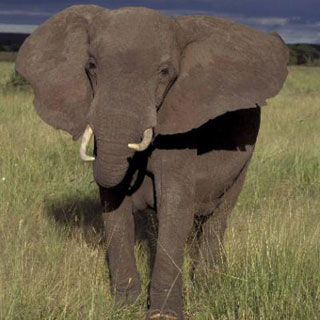
\includegraphics[width=0.8\linewidth]{elephant.jpg} % Example of an in-line image
%\end{center}

%\begin{quotation} % Example of a quotation
%\noindent{\Huge``}

%\noindent\normalsize\textit{Donec non nisl a arcu consequat varius. Sed suscipit cursus luctus. Nulla sit amet elit augue. Curabitur scelerisque mollis dolor, quis blandit lorem condimentum at.}

%\hfill{\Huge''}

%\hfill-- John Smith
%\end{quotation}

\end{multicols}

% Vorschläge für weiter Bilder:
% http://emcplus.typepad.com/.a/6a0168e71ada4c970c01901e540425970b-pi
% https://www.verifiedvoting.org/wp-content/uploads/2012/10/Internet_Voting.jpg
% https://helveticla.files.wordpress.com/2013/08/evoting.jpg?w=700
% http://www.swissinfo.ch/image/8737916/3x2/640/426/477d2f41ade9d6fa819f79c8052467e1/DG/64068625-8737920.jpg
% 

%----------------------------------------------------------------------------------------

\newpage

% --------------------------------
% THESENPAPIER PRO UND KONTRA
% --------------------------------
% Für jede These werden fünf bis sieben Sätze erwartet.


\part*{Was spricht dafür, was dagegen}

\begin{multicols}{2}
\section*{Pro}
\subsection*{Zentralisierung}
Wird digital abgestimmt, gibt es klare Zuständigkeiten für Nationale und lokale Abstimmungen. Es werden jeweils Spezialisten angestellt, welche dediziert für das E-voting verantwortlich sind und den gesamten Prozess planen, durchführen und überwachen. Das Erfassen von Kandidaten und Wählern, sowie deren Schulung, das Auswerten der Ergebnisse, wie auch das Überwachen von politischen Spenden, werden von einer zentralen Instanz koordiniert.
Dieser zentralisierte Ansatz steh im Kontrast mit den heutigen, manuellen Methoden und kann mit einer Papier-Wahl nicht realisiert werden, da jede Gemeinde und jede Stadtkreis am Abstimmungsprozess teilnimmt. Involvierte Personen kennen sich nur wenig mit dem Gesamtprozess aus und kümmern sich nur nebenbei um die Abstimmung.
 
\subsection*{Expressivität}
Lässt man alle Kombinationen einer Abstimmung zu und akzeptiert, wenn ein Wähler seine Präferenz nur für einen Kandidaten abgibt oder alle Kandidaten bewertet, lässt sich die Expressivität verschiedener Abstimmungstechnologien messen und vergleichen.
Nachweislich geben Wähler bei E-Voting mehr Präferenzen an als bei Papier. So ist die Wahrscheinlichkeit höher, dass ein Wähler seine Präferenz für alle Kandidaten abgibt als nur für seine präferierte Partei.
Ein gut gestaltetes Online-System könnte Wähler dazu motivieren nicht nur das Nötigste auszufüllen, sondern einen kompletten Wahlzettel auszufüllen. Analysedaten unterstützen die Aussage, dass ein Zusammenhang zwischen Abstimmungstechnologie und Expressivität besteht.

 
\subsection*{Einfachere Wahl für Benachteiligte}
%TODO: Dani: fertig stellen
Durch elektronische, beziehungsweise digitale, Wahlsysteme kann die Stimmabgabe für Benachteiligte erheblich vereinfacht werden. Wird kein elektronisches Wahlsystem, wie zum Beispiel i-Voting, eingesetzt, müssen Einsiedler oder Personen, welche weit entfernt vom nächsten Wahllokal leben, grosse Umstände in Kauf nehmen, um Ihre Stimme abzugeben.

Wahlkioske können zum Beispiel mit spezieller Software und Hardware ausgestattet werden, damit auch Blinde und Schwerhörige unkompliziert Ihre Stimme abgeben können.
  
\subsection*{Vereinfachte Auswertungen}
%TODO: Dani
Lorem ipsum dolor sit amet, consetetur sadipscing elitr, sed diam nonumy eirmod tempor invidunt ut labore et dolore magna aliquyam erat, sed diam voluptua. At vero eos et accusam et justo duo dolores et ea rebum. Stet clita kasd gubergren, no sea takimata sanctus est Lorem ipsum dolor sit amet. Lorem ipsum dolor sit amet, consetetur 

\subsection*{Argument 5}
Lorem ipsum dolor sit amet, consetetur sadipscing elitr, sed diam nonumy eirmod tempor invidunt ut labore et dolore magna aliquyam erat, sed diam voluptua. At vero eos et accusam et justo duo dolores et ea rebum. Stet clita kasd gubergren, no sea takimata sanctus est Lorem ipsum dolor sit amet. Lorem ipsum dolor sit amet, consetetur 

\section*{Kontra}

\subsection*{Wahlbeteiligung}
Bezüglich der Wahlbeteiligung gibt es verschiedene Ergebnisse.
Oft wird E-Voting als Gegenmassnahme zur sinkenden Wahlbeteiligung betrachtet. Dies hilft aber nur bedingt.
Während die einen, einen deutliche Anstieg dank E-Voting verzeichnen können, ist bei anderen kaum eine Änderung erkennbar.
Zwar ist bei der ersten Durchführung meistens einen Anstieg sichtbar, aber nach paar Wiederholungen, erhält man die gewohnten Werte zurück.
Wem es bei Abstimmungen wirklich um die Politik geht, der stimmt sowieso ab, sei es traditionell via Post oder modern via Internet.
Die Auseinandersetzung mit den Thema der Wahlen, wird einem auch nicht via E-Voting abgenommen.
Sprich nur der Wahlbeteiligung wegen, lohnt sich E-Voting nicht.
 
\subsection*{Betriebsausfälle und Software Bugs}
E-Voting Systeme müssen absolut ausfallsicher sein. Ein Fehler in einem solchen System hätte katastrophale Konsequenzen und würde die Sicherheit sowie die Integrität des Abstimmungssystems in Frage stellen.
Vergangene E-Votings haben gezeigt, dass selbst kleine Fehler in der Software grosse Auswirkungen haben können. Diese Auswirkungen werden möglicherweise gar nicht erkannt und die Wahl wird unwiderruflich verfälscht.
Es stellt sich die Frage, ob überhaupt sichergestellt werden kann, dass der Wahlzettel so ankommt, wie ihn der Wähler eingegeben hatte. Selbst die modernsten kryptologischen Verfahren zur Bewahrung von Vertraulichkeit und Integrität schützen nicht vor menschlichen Fehlern bei Design und Implementation von E-Voting Software.

 
\subsection*{Komplexe Aufbewahrung}
%TODO: Dani, Aufbewahrungspflicht
Für Wahldokumente besteht aufgrund ihrere rechtlichen Relevanz eine Aufbewahrungspflicht. Die Aufbewahrungspflicht ist mit diversen Auflagen verbunden. Die Auflagen müssen sowohl bei physischen als auch bei elektronischen Dokumenten erfüllt werden. Für physische Dokumente ist der Sachverhalt etwas einfacher und stellt aktuell keine grosse Herausforderung dar. Sämtliche Unterlagen und Dokumente müssen für die erforderliche Aufbewahrungsdauer vollständig, jederzeit verfügbar und fälschungssicher aufbewahrt werden. Es muss zudem sichergestellt werden, dass diese nicht gefälscht, geändert, vernichtet, gelöscht oder einzelne Informationen hinzugefügt oder entfernt werden.
Elek: Von Menschen lesbar, Portabilität Dokument, Datenschutz

Lorem ipsum dolor sit amet, consetetur sadipscing elitr, sed diam nonumy eirmod tempor invidunt ut labore et dolore magna aliquyam erat, sed diam voluptua. At vero eos et accusam et justo duo dolores et ea rebum. Stet clita kasd gubergren, no sea takimata sanctus est Lorem ipsum dolor sit amet. Lorem ipsum dolor sit amet, consetetur 
  
\subsection*{Argument 4}
Lorem ipsum dolor sit amet, consetetur sadipscing elitr, sed diam nonumy eirmod tempor invidunt ut labore et dolore magna aliquyam erat, sed diam voluptua. At vero eos et accusam et justo duo dolores et ea rebum. Stet clita kasd gubergren, no sea takimata sanctus est Lorem ipsum dolor sit amet. Lorem ipsum dolor sit amet, consetetur 

\subsection*{Argument 5}
Lorem ipsum dolor sit amet, consetetur sadipscing elitr, sed diam nonumy eirmod tempor invidunt ut labore et dolore magna aliquyam erat, sed diam voluptua. At vero eos et accusam et justo duo dolores et ea rebum. Stet clita kasd gubergren, no sea takimata sanctus est Lorem ipsum dolor sit amet. Lorem ipsum dolor sit amet, consetetur 
 
\end{multicols}

\newpage

% --------------------------------
% GLOSSAR
% --------------------------------
% Für jedenBegriff benötigen Sie vier bis sechs Sätze.


\part*{Glossar}

\begin{multicols}{2}

\subsection*{Expressivität/Expressivity}
Expressivität bestimmt wie genau ein Wähler seine effektive Präferenz in seiner Wahl wiederspiegelt. Gibt es z.B. drei Parteien mit jeweils 10 Kandidaten, welche mit einer Präferenz von 1-30 gewählt werden können, hätte ein Wahlzettel, welcher komplett ausgefüllt ist, bei jedem Namen eine Präferenz zwischen 1 und 30. Oft wird aber nur die eigene Partei gewählt und die anderen Parteien bleiben leer. Ein solcher Wahlzettel hätte nur die Präferenzen von 1-10 vergeben und somit eine geringere Expressivität.
 
\subsection*{Italian Attack}
Der 'Italian Attack' wird auch Signatur-Angriff genannt. Ein Person welche das Wahlergebnis durch Bestechung beeinflussen will, könnte Anweisungen an bestochene Wähler geben. Beispiel: Bestochene Wähler würden als erstes einen spezifischen Kandidaten wählen und dann die Nachfolgenden Präferenzen ein einer ganz speziellen Reihenfolge Wählen. Die Wahlzettel dieser bestochenen Wähler erhielten dann eine gewisse Signatur, anhand dieser der Bestecher kontrollieren könnte, wie erfolgreich seine Bestechung wahr. Dies ist nur möglich, wenn die Wahlzettel offen gelegt werden und wenn es eine hohe Anzahl an Präferenzen gibt.
 
\subsection*{Wort 3}
Lorem ipsum dolor sit amet, consetetur sadipscing elitr, sed diam nonumy eirmod tempor invidunt ut labore et dolore magna aliquyam erat, sed diam voluptua. At vero eos et accusam et justo duo dolores et ea rebum. Stet clita kasd gubergren, no sea takimata sanctus est Lorem ipsum dolor sit amet. Lorem ipsum dolor sit amet, consetetur 
  
\subsection*{Wort 4}
Lorem ipsum dolor sit amet, consetetur sadipscing elitr, sed diam nonumy eirmod tempor invidunt ut labore et dolore magna aliquyam erat, sed diam voluptua. At vero eos et accusam et justo duo dolores et ea rebum. Stet clita kasd gubergren, no sea takimata sanctus est Lorem ipsum dolor sit amet. Lorem ipsum dolor sit amet, consetetur 

\subsection*{Wort 5}
Lorem ipsum dolor sit amet, consetetur sadipscing elitr, sed diam nonumy eirmod tempor invidunt ut labore et dolore magna aliquyam erat, sed diam voluptua. At vero eos et accusam et justo duo dolores et ea rebum. Stet clita kasd gubergren, no sea takimata sanctus est Lorem ipsum dolor sit amet. Lorem ipsum dolor sit amet, consetetur 

\subsection*{Wort 6}
Lorem ipsum dolor sit amet, consetetur sadipscing elitr, sed diam nonumy eirmod tempor invidunt ut labore et dolore magna aliquyam erat, sed diam voluptua. At vero eos et accusam et justo duo dolores et ea rebum. Stet clita kasd gubergren, no sea takimata sanctus est Lorem ipsum dolor sit amet. Lorem ipsum dolor sit amet, consetetur 

\subsection*{Wort 7}
Lorem ipsum dolor sit amet, consetetur sadipscing elitr, sed diam nonumy eirmod tempor invidunt ut labore et dolore magna aliquyam erat, sed diam voluptua. At vero eos et accusam et justo duo dolores et ea rebum. Stet clita kasd gubergren, no sea takimata sanctus est Lorem ipsum dolor sit amet. Lorem ipsum dolor sit amet, consetetur 

\subsection*{Wort 8}
Lorem ipsum dolor sit amet, consetetur sadipscing elitr, sed diam nonumy eirmod tempor invidunt ut labore et dolore magna aliquyam erat, sed diam voluptua. At vero eos et accusam et justo duo dolores et ea rebum. Stet clita kasd gubergren, no sea takimata sanctus est Lorem ipsum dolor sit amet. Lorem ipsum dolor sit amet, consetetur 

\subsection*{Wort 9}
Lorem ipsum dolor sit amet, consetetur sadipscing elitr, sed diam nonumy eirmod tempor invidunt ut labore et dolore magna aliquyam erat, sed diam voluptua. At vero eos et accusam et justo duo dolores et ea rebum. Stet clita kasd gubergren, no sea takimata sanctus est Lorem ipsum dolor sit amet. Lorem ipsum dolor sit amet, consetetur 


\subsection*{Wort 10}
Lorem ipsum dolor sit amet, consetetur sadipscing elitr, sed diam nonumy eirmod tempor invidunt ut labore et dolore magna aliquyam erat, sed diam voluptua. At vero eos et accusam et justo duo dolores et ea rebum. Stet clita kasd gubergren, no sea takimata sanctus est Lorem ipsum dolor sit amet. Lorem ipsum dolor sit amet, consetetur 

\end{multicols}


\end{document}